\documentclass{standalone}
\usepackage{tikz}
\usetikzlibrary{patterns, positioning}
\usepackage[sfdefault]{ClearSans} %% option 'sfdefault' activates Clear Sans as the default text font
\usepackage[T1]{fontenc}

\begin{document}
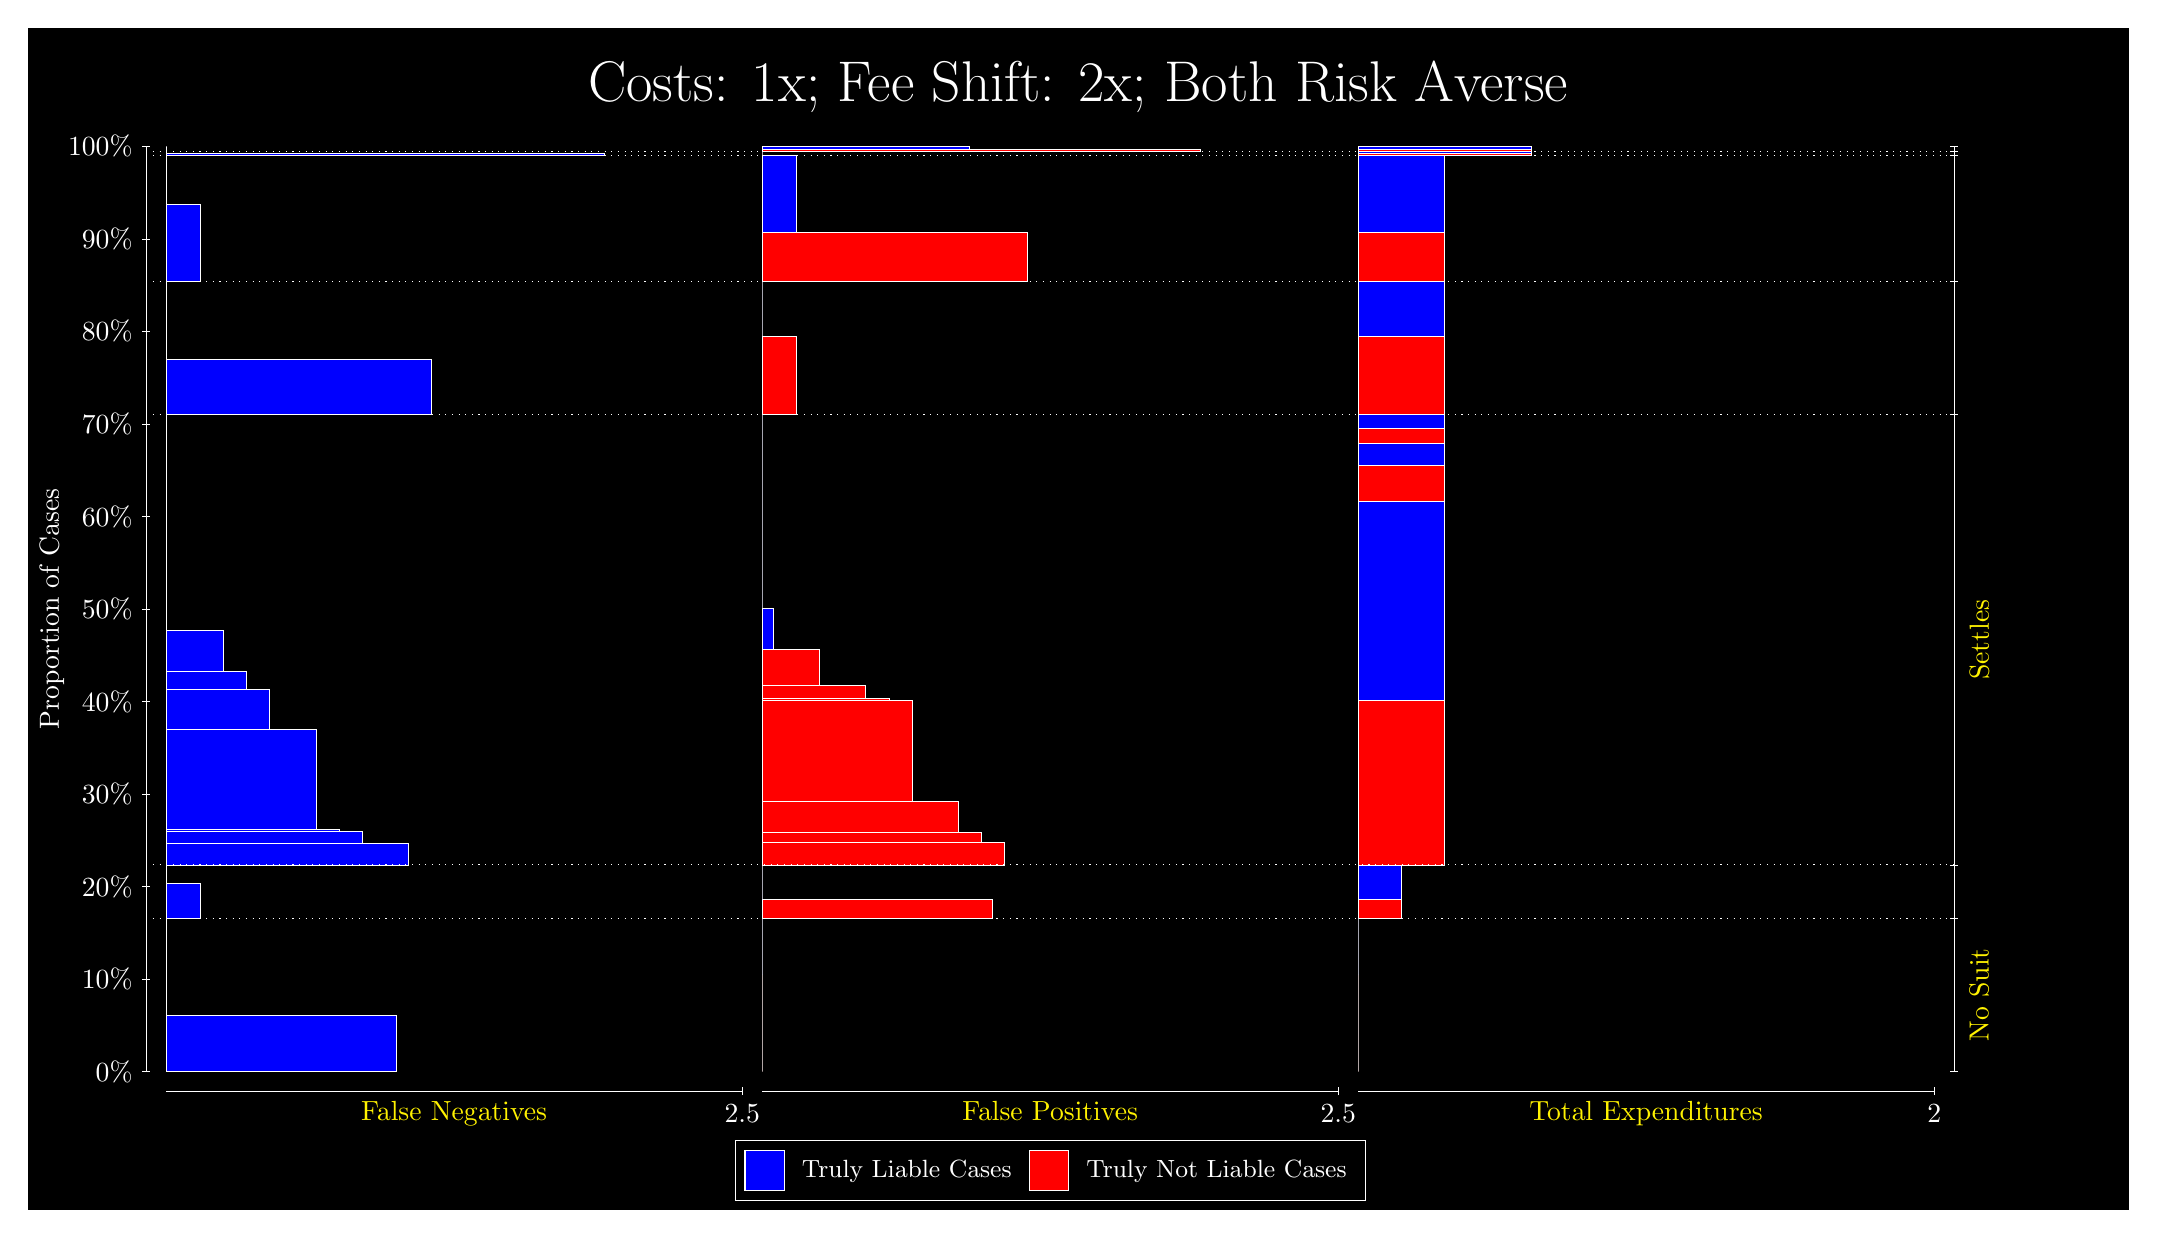
\begin{tikzpicture}
\draw[fill=black] (0,0) rectangle (26.667,15);
\draw[text=white] (0,13.5) rectangle (26.667,15) node[midway] {\huge Costs: 1x; Fee Shift: 2x; Both Risk Averse};
\draw[white, very thin] (1.5,1.75) -- (1.5,13.5);
\node[rotate=90, text=white, anchor=center] at (0.3, 7.625) {Proportion of Cases};
\draw[white, very thin] (1.45,1.75) -- (1.55,1.75);
\node[text=white, anchor=east] at (1.45, 1.75) {0\%};
\draw[white, very thin] (1.45,2.925) -- (1.55,2.925);
\node[text=white, anchor=east] at (1.45, 2.925) {10\%};
\draw[white, very thin] (1.45,4.1) -- (1.55,4.1);
\node[text=white, anchor=east] at (1.45, 4.1) {20\%};
\draw[white, very thin] (1.45,5.275) -- (1.55,5.275);
\node[text=white, anchor=east] at (1.45, 5.275) {30\%};
\draw[white, very thin] (1.45,6.45) -- (1.55,6.45);
\node[text=white, anchor=east] at (1.45, 6.45) {40\%};
\draw[white, very thin] (1.45,7.625) -- (1.55,7.625);
\node[text=white, anchor=east] at (1.45, 7.625) {50\%};
\draw[white, very thin] (1.45,8.8) -- (1.55,8.8);
\node[text=white, anchor=east] at (1.45, 8.8) {60\%};
\draw[white, very thin] (1.45,9.975) -- (1.55,9.975);
\node[text=white, anchor=east] at (1.45, 9.975) {70\%};
\draw[white, very thin] (1.45,11.15) -- (1.55,11.15);
\node[text=white, anchor=east] at (1.45, 11.15) {80\%};
\draw[white, very thin] (1.45,12.325) -- (1.55,12.325);
\node[text=white, anchor=east] at (1.45, 12.325) {90\%};
\draw[white, very thin] (1.45,13.5) -- (1.55,13.5);
\node[text=white, anchor=east] at (1.45, 13.5) {100\%};

\draw[white, very thin] (24.457,1.75) -- (24.457,13.5);
\draw[white, very thin] (24.407,1.75) -- (24.507,1.75);
\node[anchor=west] at (24.407, 1.75) {};
\draw[white, very thin] (24.407,3.6955) -- (24.507,3.6955);
\node[anchor=west] at (24.407, 3.6955) {};
\draw[white, very thin] (24.407,4.374) -- (24.507,4.374);
\node[anchor=west] at (24.407, 4.374) {};
\draw[white, very thin] (24.407,10.096) -- (24.507,10.096);
\node[anchor=west] at (24.407, 10.096) {};
\draw[white, very thin] (24.407,11.784) -- (24.507,11.784);
\node[anchor=west] at (24.407, 11.784) {};
\draw[white, very thin] (24.407,13.388) -- (24.507,13.388);
\node[anchor=west] at (24.407, 13.388) {};
\draw[white, very thin] (24.407,13.438) -- (24.507,13.438);
\node[anchor=west] at (24.407, 13.438) {};
\draw[white, very thin] (24.407,13.5) -- (24.507,13.5);
\node[anchor=west] at (24.407, 13.5) {};

\draw[white, very thin, fill=blue] (1.75,1.75) rectangle (4.6775,2.4692);
\draw[white, very thin, fill=red] (1.75,2.4692) rectangle (1.75,3.6955);
\draw[white, very thin, fill=blue] (1.75,3.6955) rectangle (2.1891,4.1349);
\draw[white, very thin, fill=red] (1.75,4.1349) rectangle (1.75,4.374);
\draw[white, very thin, fill=blue] (1.75,4.374) rectangle (4.8239,4.6482);
\draw[white, very thin, fill=blue] (1.75,4.6482) rectangle (4.2384,4.802);
\draw[white, very thin, fill=blue] (1.75,4.802) rectangle (3.9457,4.8228);
\draw[white, very thin, fill=blue] (1.75,4.8228) rectangle (3.6529,6.1012);
\draw[white, very thin, fill=blue] (1.75,6.1012) rectangle (3.0674,6.6075);
\draw[white, very thin, fill=blue] (1.75,6.6075) rectangle (2.7746,6.8331);
\draw[white, very thin, fill=blue] (1.75,6.8331) rectangle (2.4819,7.3544);
\draw[white, very thin, fill=red] (1.75,7.3544) rectangle (1.75,10.096);
\draw[white, very thin, fill=blue] (1.75,10.096) rectangle (5.1167,10.795);
\draw[white, very thin, fill=red] (1.75,10.795) rectangle (1.75,11.784);
\draw[white, very thin, fill=blue] (1.75,11.784) rectangle (2.1891,12.763);
\draw[white, very thin, fill=red] (1.75,12.763) rectangle (1.75,13.388);
\draw[white, very thin, fill=blue] (1.75,13.388) rectangle (7.3123,13.411);
\draw[white, very thin, fill=red] (1.75,13.411) rectangle (1.75,13.438);
\draw[white, very thin, fill=red] (1.75,13.438) rectangle (1.75,13.465);
\draw[white, very thin, fill=blue] (1.75,13.465) rectangle (1.75,13.5);
\draw[white, very thin, fill=red] (9.3189,1.75) rectangle (9.3189,2.9763);
\draw[white, very thin, fill=blue] (9.3189,2.9763) rectangle (9.3189,3.6955);
\draw[white, very thin, fill=red] (9.3189,3.6955) rectangle (12.246,3.9346);
\draw[white, very thin, fill=blue] (9.3189,3.9346) rectangle (9.3189,4.374);
\draw[white, very thin, fill=red] (9.3189,4.374) rectangle (12.393,4.6616);
\draw[white, very thin, fill=red] (9.3189,4.6616) rectangle (12.1,4.7899);
\draw[white, very thin, fill=red] (9.3189,4.7899) rectangle (11.807,5.1873);
\draw[white, very thin, fill=red] (9.3189,5.1873) rectangle (11.222,6.4646);
\draw[white, very thin, fill=red] (9.3189,6.4646) rectangle (10.929,6.487);
\draw[white, very thin, fill=red] (9.3189,6.487) rectangle (10.636,6.6601);
\draw[white, very thin, fill=red] (9.3189,6.6601) rectangle (10.051,7.1153);
\draw[white, very thin, fill=blue] (9.3189,7.1153) rectangle (9.4652,7.6367);
\draw[white, very thin, fill=blue] (9.3189,7.6367) rectangle (9.3189,10.096);
\draw[white, very thin, fill=red] (9.3189,10.096) rectangle (9.758,11.085);
\draw[white, very thin, fill=blue] (9.3189,11.085) rectangle (9.3189,11.784);
\draw[white, very thin, fill=red] (9.3189,11.784) rectangle (12.686,12.409);
\draw[white, very thin, fill=blue] (9.3189,12.409) rectangle (9.758,13.388);
\draw[white, very thin, fill=red] (9.3189,13.388) rectangle (9.3189,13.415);
\draw[white, very thin, fill=blue] (9.3189,13.415) rectangle (9.3189,13.438);
\draw[white, very thin, fill=red] (9.3189,13.438) rectangle (14.881,13.465);
\draw[white, very thin, fill=blue] (9.3189,13.465) rectangle (11.954,13.5);
\draw[white, very thin, fill=red] (16.888,1.75) rectangle (16.888,2.9763);
\draw[white, very thin, fill=blue] (16.888,2.9763) rectangle (16.888,3.6955);
\draw[white, very thin, fill=red] (16.888,3.6955) rectangle (17.437,3.9346);
\draw[white, very thin, fill=blue] (16.888,3.9346) rectangle (17.437,4.374);
\draw[white, very thin, fill=red] (16.888,4.374) rectangle (17.986,6.4646);
\draw[white, very thin, fill=blue] (16.888,6.4646) rectangle (17.986,8.9963);
\draw[white, very thin, fill=red] (16.888,8.9963) rectangle (17.986,9.4515);
\draw[white, very thin, fill=blue] (16.888,9.4515) rectangle (17.986,9.7257);
\draw[white, very thin, fill=red] (16.888,9.7257) rectangle (17.986,9.9211);
\draw[white, very thin, fill=blue] (16.888,9.9211) rectangle (17.986,10.096);
\draw[white, very thin, fill=red] (16.888,10.096) rectangle (17.986,11.085);
\draw[white, very thin, fill=blue] (16.888,11.085) rectangle (17.986,11.784);
\draw[white, very thin, fill=red] (16.888,11.784) rectangle (17.986,12.409);
\draw[white, very thin, fill=blue] (16.888,12.409) rectangle (17.986,13.388);
\draw[white, very thin, fill=red] (16.888,13.388) rectangle (19.083,13.415);
\draw[white, very thin, fill=blue] (16.888,13.415) rectangle (19.083,13.438);
\draw[white, very thin, fill=red] (16.888,13.438) rectangle (19.083,13.465);
\draw[white, very thin, fill=blue] (16.888,13.465) rectangle (19.083,13.5);
\draw[white, dotted] (1.5,3.6955) -- (24.457,3.6955);
\draw[white, dotted] (1.5,4.374) -- (24.457,4.374);
\draw[white, dotted] (1.5,10.096) -- (24.457,10.096);
\draw[white, dotted] (1.5,11.784) -- (24.457,11.784);
\draw[white, dotted] (1.5,13.388) -- (24.457,13.388);
\draw[white, dotted] (1.5,13.438) -- (24.457,13.438);
\draw[white, very thin] (1.75,1.5) -- (9.0689,1.5);
\node[text=yellow, anchor=north] at (5.4094, 1.5) {False Negatives};
\draw[white, very thin] (9.0689,1.45) -- (9.0689,1.55);
\node[text=white, anchor=north] at (9.0689, 1.45) {2.5};

\draw[white, very thin] (9.3189,1.5) -- (16.638,1.5);
\node[text=yellow, anchor=north] at (12.978, 1.5) {False Positives};
\draw[white, very thin] (16.638,1.45) -- (16.638,1.55);
\node[text=white, anchor=north] at (16.638, 1.45) {2.5};

\draw[white, very thin] (16.888,1.5) -- (24.207,1.5);
\node[text=yellow, anchor=north] at (20.547, 1.5) {Total Expenditures};
\draw[white, very thin] (24.207,1.45) -- (24.207,1.55);
\node[text=white, anchor=north] at (24.207, 1.45) {2};

\node[text=yellow, centered, rotate=90] at (24.777, 2.7228) {No Suit};

\node[text=yellow, centered, rotate=90] at (24.777, 7.2349) {Settles};





\draw (12.978300999999998,1.5) node[draw=none] (baseCoordinate) {};
\begin{scope}[align=center]
        \matrix[scale=0.5, draw=white, below=0.5cm of baseCoordinate, nodes={draw}, column sep=0.1cm]{
            \node[rectangle, draw, minimum width=0.5cm, minimum height=0.5cm, fill=blue] {}; &
            \node[draw=none, font=\small, text=white] (B) {Truly Liable Cases}; &
            \node[rectangle, draw, minimum width=0.5cm, minimum height=0.5cm, fill=red] {}; &
            \node[draw=none, font=\small, text=white] (B) {Truly Not Liable Cases}; \\
            };
\end{scope}

\end{tikzpicture}
\end{document}